\section{Java Sample applications}
\label{sec:JavaSampleApps}

The first two examples in this section are simple applications developed in COMPSs to easily illustrate how to code,
compile and run COMPSs applications. These applications are executed locally and show different ways to take advantge
of all the COMPSs features. 

The rest of the examples are more elaborated and consider the execution in a cloud platform where the VMs mount a common 
storage on \textbf{/sharedDisk} directory. This is useful in the case of applications that require working 
with big files, allowing to transfer data only once, at the beginning of the execution, and to enable 
the application to access the data directly during the rest of the execution.

The Virtual Machine available at our webpage (\url{http://compss.bsc.es/}) provides a development environment with
all the applications listed in the following sections. The codes of all the applications can be found under the 
$/home/compss/workspace\_java/$ folder. 

%%%%%%%%%%%%%%%
%% HELLO WORLD 
%%%%%%%%%%%%%%%
\subsection{Hello World}
The Hello Wolrd is a Java application that creates a task and prints a Hello World! message. Its purpose is to clarify that the COMPSs tasks output is
redirected to the job files and it is \textbf{not} available at the standard output. 

Next we provide the important parts of the application's code.

\begin{lstlisting}[language=java]
	// hello.Hello
	
	public static void main(String[] args) throws Exception {
		// Check and get parameters
		if (args.length != 0) {
			usage();
			throw new Exception("[ERROR] Incorrect number of parameters");
		}
		
		// Hello World from main application
		System.out.println("Hello World! (from main application)");

		// Hello World from a task
		HelloImpl.sayHello();
	}
\end{lstlisting}

As shown in the main code, this application has no input arguments. 

\begin{lstlisting}[language=java]
	// hello.HelloImpl
	
	public static void sayHello() {
		System.out.println("Hello World! (from a task)");
	}
\end{lstlisting}

Remember that, to run with COMPSs, java applications must provide an interface. For simplicity, in this example, the content of the interface only
declares the task which has no parameters:
\begin{lstlisting}[language=java]
	// hello.HelloItf
	
	@Method(declaringClass = "hello.HelloImpl")
	void sayHello(
	);
\end{lstlisting}

Notice that there is a first Hello World message printed from the main code and, a second one, printed inside a task. When executing sequentially
this application users will be able to see both messages at the standard output. However, when executing this application with COMPSs, users will only
see the message from the main code at the standard output. The message printed from the task will be stored inside the job log files. 

Let's try it. First we proceed to compile the code by running the following instructions:

\begin{lstlisting}[language=bash]
compss@bsc:~$ cd ~/workspace_java/hello/src/
compss@bsc:~$ javac *.java

\end{lstlisting}

Once done, we can sequentially execute the application by directly invoking the \textit{jar} file.

\begin{lstlisting}[language=bash]
compss@bsc:~$ java -jar hello.jar
\end{lstlisting}

And we can also execute the application with COMPSs:

\begin{lstlisting}[language=bash]
compss@bsc:~$ cd ~/workspace_java/hello/jar/
compss@bsc:~/workspace_java/hello/jar$ runcompss -d hello.Hello 
\end{lstlisting}

Notice that the COMPSs execution is using the \textit{-d} option to allow the job logging. Thus, we can check out the application jobs folder to look for
the task output.

\begin{lstlisting}[language=bash]
compss@bsc:~$ cd ~/.COMPSs/hello.Hello_01/jobs/
compss@bsc:~/.COMPSs/hello.Hello_01/jobs$ ls -1

compss@bsc:~/.COMPSs/hello.Hello_01/jobs$ cat job1_NEW.out

\end{lstlisting}

%%%%%%%%%%%%%%%
%% SIMPLE
%%%%%%%%%%%%%%%
\subsection{Simple}
The Simple application is a Java application that increases a counter by means of a task. The counter is stored inside a file.


%%%%%%%%%%%%%%%
%% Increment
%%%%%%%%%%%%%%%
\subsection{Increment}
The Increment application is a Java application that increases N time three different counters. Each increase step is developed by a separated task. The
purpose of this application is to show parallelism between the three counters.

Next we provide the main code of this application. The code inside the \textit{increment} task is the same than the previous example. 

\begin{lstlisting}[language=java]
	// increment.Increment
	
\end{lstlisting}

As shown in the main code, this application has 4 parameters that stand for:

\begin{enumerate}
 \item \textbf{N:} Number of times to increase a counter
 \item \textbf{InitialValue1:} Initial value for counter 1
 \item \textbf{InitialValue2:} Initial value for counter 2
 \item \textbf{InitialValue3:} Initial value for counter 3
\end{enumerate}

Next we will compile and run the Increment application with the \textit{-g} option to be able to generate the final graph at the end of the execution.

\begin{lstlisting}[language=bash]
compss@bsc:~$ cd ~/workspace_java/increment/jar/
compss@bsc:~/workspace_java/increment/jar$ runcompss -g increment.Increment 10 1 2 3 

compss@bsc:~/workspace_java/increment/jar$ cd ~/.COMPSs/increment.Increment_01/monitor/
compss@bsc:~/.COMPSs/increment.Increment_01/monitor$ gengraph complete_graph.dot
compss@bsc:~/.COMPSs/increment.Increment_01/monitor$ evince complete_graph.dot.pdf
\end{lstlisting}

%%%%%%%%%%%%%%%
%% MATMUL
%%%%%%%%%%%%%%%
\subsection{Matrix multiplication}
The Matrix Multiplication (Matmul) is a pure Java application that multiplies two matrices in a direct way. 
The application creates 2 matrices of N x N size initialized with values, and multiply the matrices by blocks.

\begin{figure}[ht!]
  \centering
    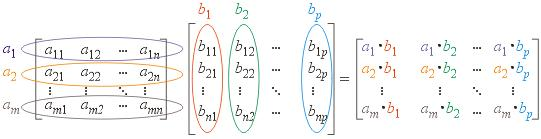
\includegraphics[width=0.8\textwidth]{./Sections/2_Java/Figures/matrix.jpeg}
    \caption{Matrix multiplication} 
    \label{fig:matrix}
\end{figure}

In this application the multiplication is implemented in the multiplyAccumulative that is thus selected 
as the task that will be executed remotely. In order to run the application the matrix dimension (number of blocks) and the dimension of each block
have to be supplied.

\begin{lstlisting}[language=bash]
compss@bsc:~$ cp ~/workspace_java/matmul/package/Matmul.tar.gz /home/compss/
compss@bsc:~$ tar xzf Matmul.tar.gz
\end{lstlisting}

The command line to execute the application:

\begin{lstlisting}[language=bash]
compss@bsc:~$ runcompss matmul.Matmul <matrix_dim> <block_dim>
\end{lstlisting}

%%%%%%%%%%%%%%%
%% SPARSELU 
%%%%%%%%%%%%%%%
\subsection{Sparse LU decomposition}
SparseLU multiplies two matrices using the factorization method of LU decomposition, which factorizes a 
matrix as a product of a lower triangular matrix and an upper one.

\begin{figure}[ht!]
  \centering
    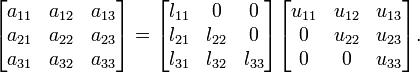
\includegraphics[width=0.6\textwidth]{./Sections/2_Java/Figures/SparseLU.jpeg}
    \caption{Sparse LU decomposition}
    \label{fig:SparseLO}
\end{figure}

The matrix is divided into N x N blocks on where 4 types of operations will be applied modifying the blocks: 
{\bf lu0}, {\bf fwd}, {\bf bdiv} and {\bf bmod}. These four operations are implemented in four methods that 
are selecetd as the tasks that will be executed remotely. In order to run the application the matrix dimension 
has to be provided.

\begin{lstlisting}[language=bash]
compss@bsc:~$ cp ~/workspace/sparselu/package/SparseLU.tar.gz /home/compss/
compss@bsc:~$ tar xzf SparseLU.tar.gz
\end{lstlisting}

The command line to execute the application:

\begin{lstlisting}[language=bash]
compss@bsc:~$ runcompss sparselu.SparseLU <matrix_dim>
\end{lstlisting}


%%%%%%%%%%%%%%%
%% KMEANS
%%%%%%%%%%%%%%%
\subsection{KMeans}


%%%%%%%%%%%%%%%
%% BLAST
%%%%%%%%%%%%%%%
\subsection{BLAST Workflow}
BLAST is a widely-used bioinformatics tool for comparing primary biological sequence information, such as 
the amino-acid sequences of different proteins or the nucleotides of DNA sequences with sequence databases, 
identifying sequences that resemble the query sequence above a certain threshold. 
The work performed by the COMPSs Blast workflow is computationally intensive and embarrassingly parallel.

\begin{figure}[ht!]
  \centering
    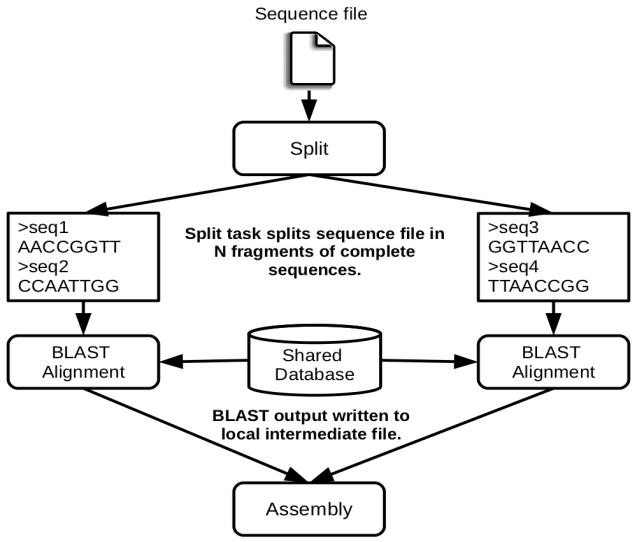
\includegraphics[width=0.7\textwidth]{./Sections/2_Java/Figures/blast_workflow.jpeg}
    \caption{The COMPSs Blast workflow}
    \label{fig:BLAST_workflow}
\end{figure}

The workflow describes the three blocks of the workflow implemented in the {\bf Split}, {\bf Align} and 
{\bf Assembly} methods. The second one is the only method that is chosen to be executed remotely, so it 
is the unique method defined in the interface file. The {\bf Split} method chops the query sequences file 
in N fragments, {\bf Align} compares each sequence fragment against the database by means of the Blast 
binary, and {\bf Assembly} combines all intermediate files into a single result file.

This application uses a database that will be on the shared disk space avoiding transferring the entire 
database (which can be large) between the virtual machines.

\begin{lstlisting}[language=bash]
compss@bsc:~$ cp ~/workspace/blast/package/Blast.tar.gz /home/compss/
compss@bsc:~$ tar xzf Blast.tar.gz
\end{lstlisting}

The command line to execute the workflow:

\begin{lstlisting}[language=bash]
compss@bsc:~$ runcompss blast.Blast <debug> 
                                    <bin_location>
                                    <database_file> 
                                    <sequences_file>
                                    <frag_number> 
                                    <tmpdir>
                                    <output_file>
\end{lstlisting}

Where:
\begin{itemize}
 \item {\bf debug}: The debug flag of the application (true or false).
 \item {\bf bin\_location}: Path of the Blast binary.
 \item {\bf database\_file}: Path of database file; the shared disk {\bf /sharedDisk/} is suggested to avoid big data transfers.
 \item {\bf sequences\_file}: Path of sequences file.
 \item {\bf frag\_number}: Number of fragments of the original sequence file, this number determines the number of parallel Align tasks.
 \item {\bf tmpdir}: Temporary directory ({\bf /home/compss/tmp/}).
 \item {\bf output\_file}: Path of the result file.
\end{itemize}
 
Example:
\begin{lstlisting}[language=bash]
compss@bsc:~$ runcompss blast.Blast true
                        /home/compss/workspace_java/blast/binary/blastall
                        /sharedDisk/Blast/databases/swissprot/swissprot
                        /sharedDisk/Blast/sequences/sargasso_test.fasta 
                        4 
                        /tmp/
                        /home/compss/out.txt
\end{lstlisting}